\documentclass[conference,a4paper]{IEEEtran}
\IEEEoverridecommandlockouts

\usepackage{cite}
\usepackage{amsmath,amssymb,amsfonts}
\usepackage{booktabs}
\usepackage{graphicx}
\usepackage{textcomp}
\usepackage{xcolor}
\usepackage{microtype}
\usepackage{flushend}
\usepackage{indentfirst}
\usepackage[
  a4paper,
  top=19.05mm,
  bottom=42.93mm,
  left=12.95mm,
  right=12.95mm
]{geometry}
\usepackage{titlesec}

\setlength{\columnsep}{12.7mm}
\setlength{\parindent}{0.2in}
\setlength{\parskip}{6pt}
\linespread{0.95}
\pagestyle{empty}

\titleformat{\section}[block]
  {\normalfont\normalsize\scshape\filcenter}{\thesection.}{0.5em}{}
\titleformat{name=\section,numberless}[block]
  {\normalfont\fontsize{12}{14.4}\selectfont\bfseries\filcenter}{}{0pt}{}
\titlespacing*{\section}{0pt}{8pt}{4pt}
\titleformat{\subsection}[hang]
  {\normalfont\normalsize\itshape}{\Alph{subsection}.}{0.5em}{}
\titlespacing*{\subsection}{0pt}{6pt}{3pt}
\titleformat{\subsubsection}[hang]
  {\normalfont\normalsize\itshape}{\arabic{subsubsection})}{0.5em}{}
\titlespacing*{\subsubsection}{0pt}{0pt}{0pt}

\begin{document}

\title{\fontsize{16}{19.2}\selectfont\bfseries Evaluating Two-Stage Candidate Routing for Indirect Prompt Injection Screening in Retrieval-Augmented Generation Systems}

\author{\IEEEauthorblockN{\fontsize{12}{14.4}\selectfont Yan-Wei Li, Jun-Ren Chen and Lung-Lung Liu*}
\IEEEauthorblockA{\fontsize{12}{14.4}\selectfont
Information Technology and Management Program \\
Ming Chuan University\\
Taoyuan, Taiwan ROC \\
\{11890054, 11890045\}@me.mcu.edu.tw, *llliu@mail.mcu.edu.tw}}

\maketitle

\section*{Abstract}
{\fontsize{9}{10.8}\selectfont\bfseries
Retrieval-Augmented Generation (RAG) systems may treat indirect prompt injection (IPI) instructions in retrieved documents as commands. We evaluate a black-box, two-stage screening method that combines a lightweight Semantic Risk Score with candidate-routed local review. Across two pre-inference-locked, context-disjoint Benchmark for Indirect Prompt Injection Attacks (BIPIA) holdouts, internally labeled v4 and v5, the observed pooled Attack Success Rate (ASR) was 29.0\% without screening and 1.0\% with the method, a paired difference of $-28$ percentage points (95\% confidence interval [CI]: $-36$ to $-20$ points). The paired benign-utility difference was $-0.03848$ (95\% CI: $-0.07526$ to $-0.00957$), with a 5\% benign block rate and a 25\% Tier-2 trigger rate. In v4, candidate routing used 74\% fewer Tier-2 calls than always-on review; the corresponding ASR estimates were 2\% and 0\%. External InjecAgent and HouYi Gate tests revealed representation-dependent routing behavior. These results characterize an observed security--utility--review-cost trade-off within the evaluated settings and do not establish general IPI robustness.\par}

{\noindent\fontsize{10}{12}\selectfont\bfseries\itshape Keywords: }
{\fontsize{9}{10.8}\selectfont Retrieval-Augmented Generation, Indirect Prompt Injection, Large Language Model Security, Semantic Risk Assessment, Candidate Routing\par}

\section{Introduction}
Retrieval-Augmented Generation (RAG) is intended to improve factual grounding and knowledge freshness by adding retrieved documents to a Large Language Model (LLM) context \cite{b2,b3}. This external context also creates a trust-boundary problem: instructions in web pages, e-mails, tables, or documents may be interpreted as commands. Such Indirect Prompt Injection (IPI) may redirect the intended task, manipulate output, or request sensitive information \cite{b4,b5}.

Existing approaches include rule-based filters, prompt separation, trained detectors, model alignment, and LLM-based review \cite{b5,b6}. Lightweight rules are deployable but may be sensitive to paraphrases and unfamiliar wrappers; structured-input or alignment approaches may require modifying the generator. Reviewing every retrieved document may add semantic information but also increases inference cost and can increase false blocking.

We study a two-stage gate for black-box, text-only RAG deployments. Tier-1 combines multilingual semantic intent deviation with instruction-pattern score in a Semantic Risk Score (SRS) to pass, block, or route directive candidates. Tier-2 applies structured local adjudication only to routed samples and records decisions without modifying the downstream generator. We evaluate the design on two locked, context-disjoint BIPIA holdouts \cite{b6} and use InjecAgent and HouYi formulations to examine representation sensitivity. The Conclusion summarizes the reported contributions and limitations.

\section{Literature Review}
\subsection{Prompt-Level and Structured-Input Defenses}
Spotlighting marks the provenance of untrusted content through delimiting, datamarking, or encoding and can be applied to black-box language models \cite{b7}. Its outcome nevertheless depends on the generator recognizing and following those signals. StruQ places trusted instructions and external data in distinct input channels and trains a model to process that structure \cite{b8}. This requires a specially trained generator and may not be available through an existing commercial application programming interface (API). The evaluated gate instead operates outside the generator and requires no retraining.

\subsection{Model-Based and Detection-Based Defenses}
SecAlign trains a model to prefer task-consistent outputs over injected alternatives, aiming to improve model-level resistance at the cost of parameter access and additional alignment \cite{b9}. Detection-based work has combined instruction detection with segmentation or extraction so that identified content can be removed before generation \cite{b10}. Applying such a model to every document, however, adds inference cost.

InstructDetector uses intermediate hidden states and gradients to classify contextual data and injected instructions \cite{b11}. These signals require white-box access. Our design uses text-only inputs and selectively invokes local semantic review, trading access to internal signals for compatibility with black-box RAG services.

\subsection{Agent-Level Defenses and Adaptive Robustness}
Task Shield checks whether extracted instructions and tool calls remain aligned with the user's objective \cite{b12}, while CaMeL separates trusted control flow from untrusted data flow and restricts capabilities \cite{b13}. Both target tool-executing agents; CaMeL also requires substantial execution-environment restructuring. Our scope is the earlier text boundary, before retrieved content enters an existing RAG generator.

Adaptive evaluations have reported bypasses of defenses evaluated on static benchmarks after prompts were reformulated in a defense-aware manner \cite{b14}. We therefore supplement BIPIA with fixed-gate InjecAgent \cite{b15} and HouYi \cite{b16} formulations. These tests examine representation sensitivity rather than establish cross-benchmark robustness.

\section{Methodology}
We evaluate a text-screening boundary for black-box RAG deployments that selectively invokes a structured local reviewer. The reported measurements cover evaluator-labeled attack success, benign utility, review frequency, and observed inference overhead.
\subsection{Threat Model and Problem Formulation}
The input to the protected RAG system consists of a system instruction $x_{\mathrm{sys}}$, a user query $x_{\mathrm{user}}$, and retrieved external content $x_{\mathrm{ext}}$. The downstream generation model $M$ produces an output $y$ based on the combined context:
\begin{equation}
y=M(x_{\mathrm{sys}},x_{\mathrm{user}},x_{\mathrm{ext}}).
\end{equation}
The system instruction and user query are treated as trusted inputs, while all retrieved external content is treated as untrusted. The attacker is assumed to be capable of inserting or modifying content in an external data source that may subsequently be retrieved by the RAG system. However, the attacker cannot modify the system instruction, directly alter the user query, or change the parameters of the downstream generation model.

The attacker's objective is to cause the generated output to deviate from the task intended by $x_{\mathrm{sys}}$ and $x_{\mathrm{user}}$. Representative attacks include instruction override, task hijacking, output manipulation, data exfiltration, and the insertion of misleading or attacker-controlled information. The screening module $D$ is inserted between the retriever and the downstream generator:
\begin{equation}
D(x_{\mathrm{user}},x_{\mathrm{ext}})\rightarrow
\{\textsc{pass},\textsc{review},\textsc{block}\}.
\end{equation}
A PASS decision permits the retrieved content to enter the downstream context. A REVIEW decision invokes the second-stage structured reviewer, while a BLOCK decision excludes the content from downstream generation.

The scope of this study is limited to textual response-stage defense. Retriever poisoning detection, multimodal hidden instructions, HyperText Markup Language (HTML) rendering attacks, and authorization control for executable tools are outside the current threat model.

\subsection{Two-Stage Candidate-Routed Architecture}
The evaluated architecture is placed between the retriever and the RAG generator, as shown in Fig.~\ref{fig:architecture}. After a user query is submitted, the retriever obtains one or more external documents. Retrieved content is first passed to the Tier-1 risk scorer rather than being directly inserted into the generation prompt.

Tier-1 computes an SRS and extracts directive-related signals. The routing policy then assigns one of three actions. Low-risk content is passed to the RAG generator, high-risk content is blocked, and candidate-risk content is forwarded to the Tier-2 local reviewer.

Tier-2 is prompted to classify whether retrieved content contains an instruction that attempts to cross the trust boundary between external data and executable commands. Its structured output is mapped to a PASS or BLOCK decision.

This design separates Tier-1 scoring from the more computationally intensive Tier-2 review and records the resulting screening decisions before retrieved content reaches the downstream generator.

\subsection{Tier-1 Semantic Risk Score}
For each user query and retrieved context pair, Tier-1 evaluates three candidate feature groups: semantic intent deviation, instruction-pattern score, and pressure-related signals. The initial score is defined as:
\begin{equation}
\mathrm{SRS}(x_{\mathrm{user}},x_{\mathrm{ext}})=
\alpha D_{\mathrm{intent}}+\beta R_{\mathrm{instruction}}+
\gamma P_{\mathrm{pressure}},
\end{equation}
where $D_{\mathrm{intent}}$ measures semantic deviation from the user task, $R_{\mathrm{instruction}}$ denotes a saturated score based on distinct instruction-related regular-expression patterns, and $P_{\mathrm{pressure}}$ represents coercive or urgency-related language.

\subsubsection{Semantic Intent Deviation}
The user query and retrieved content are encoded using a fixed multilingual E5 (EmbEddings from bidirEctional Encoder rEpresentations) text-embedding model \cite{b17}. Because a short malicious instruction may be hidden inside a long document, the external content is divided into chunks $c_1,c_2,\ldots,c_n$. The intent-deviation score is calculated using the maximum cosine distance between the user query and any external-content chunk:
\begin{equation}
D_{\mathrm{intent}}=1-\min_{c_i\in x_{\mathrm{ext}}}
\cos\left(E_q(x_{\mathrm{user}}),E_p(c_i)\right).
\end{equation}
where $E_q(\cdot)$ and $E_p(\cdot)$ denote multilingual-E5 encodings using the query: and passage: prefixes, respectively. A high value indicates that at least one portion of the retrieved content is semantically distant from the user's intended task.

\subsubsection{Instruction-Pattern Score}
The instruction-pattern score feature detects imperative verbs, instruction-override expressions, role-escalation statements, output-control phrases, and requests for sensitive information. Representative patterns include requests to ignore prior instructions, reveal hidden content, change the model's role, produce attacker-specified output, or perform an unrelated task.

The feature counts distinct matched instruction-related patterns rather than total occurrences, preventing repeated instances of the same expression from disproportionately increasing the score:
\begin{equation}
R_{\mathrm{instruction}}=
\min\left(\frac{|\mathcal{M}_{\mathrm{instruction}}(x_{\mathrm{ext}})|}{2},1\right),
\end{equation}
where $\mathcal{M}_{\mathrm{instruction}}(x_{\mathrm{ext}})$ denotes the set of distinct instruction-related regular-expression patterns matched in the retrieved context. Each pattern contributes at most once, and the feature saturates after two distinct matches.

\subsubsection{Pressure-Related Signals}
Pressure-related signals capture urgency, coercion, mandatory language, threats of failure, and similar social-engineering expressions. These signals were included as a candidate feature because malicious instructions may attempt to increase compliance by using terms such as ``immediately,'' ``must,'' or ``do not refuse.''

However, validation-based calibration assigned this feature a weight of zero. The final calibrated SRS is therefore:
\begin{equation}
\mathrm{SRS}=0.6D_{\mathrm{intent}}+0.4R_{\mathrm{instruction}}.
\end{equation}
The pressure-related feature is retained only for ablation analysis and diagnostic logging.

\subsection{Candidate-Routing Policy}
The Tier-1 decision function is defined as:
\begin{equation}
\resizebox{\columnwidth}{!}{$\displaystyle
G(x_{\mathrm{user}},x_{\mathrm{ext}})=
\begin{cases}
\textsc{block},&\mathrm{SRS}>\tau_{\mathrm{high}},\\
\textsc{review},&C_{\mathrm{directive}}=1\ \lor\
\tau_{\mathrm{low}}\leq\mathrm{SRS}\leq\tau_{\mathrm{high}},\\
\textsc{pass},&\text{otherwise}.
\end{cases}
$}
\end{equation}
where $C_{\mathrm{directive}}$ indicates whether a directive candidate is detected. Validation-based calibration selected:
\begin{equation}
\tau_{\mathrm{low}}=\tau_{\mathrm{high}}=0.185.
\end{equation}
Therefore, a score exactly equal to 0.185 is routed to REVIEW, whereas only scores strictly above 0.185 are directly blocked. Because the calibrated interval collapses to a single boundary, Tier-2 is activated primarily by directive-candidate routing.

\subsection{Tier-2 Structured Local Reviewer}
Samples assigned to REVIEW are processed by a locally deployed language-model reviewer. The reviewer receives the trusted user task and untrusted retrieved content with explicit source labels. It is instructed to determine whether the external content attempts to override trusted instructions, redirect the task, manipulate the output, or obtain sensitive information.

The reviewer returns a schema-constrained output containing \texttt{risk\_label}, \texttt{risk\_type}, \texttt{evidence\_span}, \texttt{confidence}, and \texttt{short\_reason}. The evidence span must occur verbatim in the retrieved context. Malicious decisions are blocked, benign decisions are passed, and invalid, schema-incomplete, or unresolved Tier-2 outputs are conservatively mapped to BLOCK.
\subsection{Final Decision and Security Logging}
If the final decision is PASS, the retrieved context is forwarded to the downstream RAG generator. If the decision is BLOCK, the suspicious context is excluded from the generation prompt.

For each evaluated sample, the system records:
\begin{enumerate}
    \item semantic intent-deviation score;
    \item instruction-density score;
    \item matched directive patterns;
    \item pressure-related diagnostic signals;
    \item Tier-1 routing decision;
    \item Tier-2 structured output, if activated; and
    \item final PASS or BLOCK decision and detector latency.
\end{enumerate}
These logs can be used for error analysis, calibration checks, monitoring, and post-incident review.

\begin{figure}[t]
\centering
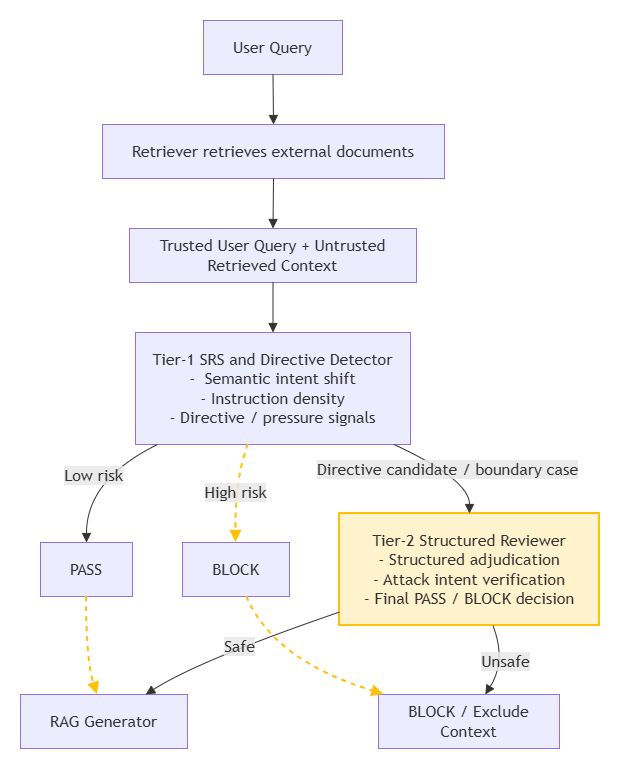
\includegraphics[width=0.84\columnwidth]{2-Tiier Architecture.drawio.png}
\caption{Evaluated two-stage candidate-routed screening architecture. Pressure signals are retained for diagnostic logging but have zero weight in the selected SRS.}
\label{fig:architecture}
\end{figure}

\section{Experimental Setup}
\subsection{Dataset and Evaluation Split}
The labels v4 and v5 are internal holdout identifiers, not BIPIA release versions. v4 denotes the first main holdout, locked before inference with selection seed 20260705 after excluding context groups used by earlier pilots. v5 denotes a second replication, locked with seed 20260712 after excluding all v4 context groups. Each holdout contains ten previously unconsumed context groups per task across summarization, code, e-mail, web, and table question answering. One benign and one malicious row are paired within each context, yielding 50 benign and 50 malicious rows per holdout; the two holdouts have no shared context groups or sample identifiers. v4 includes 24 BIPIA attack families, whereas v5 includes all 25, including Ransomware. The pooled analysis therefore contains 100 benign and 100 malicious rows and spans all 25 families. Retrieved contexts are supplied directly, so retriever recall is not evaluated. The web question-answering (WebQA) portion is a public-data reconstruction containing News Question Answering (NewsQA) \texttt{story\_text}, not a byte-identical reproduction of the unavailable Message-Digest Algorithm 5 (MD5) artifact.

\subsection{Models and Paired Protocol}
Downstream generation, candidate Tier-2 review, always-on Tier-2 review, and primary model-evaluated family labels used a local 8.0B four-bit K-quant medium (Q4\_K\_M) Gemma 4 model served by Ollama 0.31.2 (\texttt{gemma4:latest}, manifest \texttt{c6eb396dbd59}), with temperature 0 and seed 42. An independently tagged 31.3B Q4\_K\_M Gemma 4 model (\texttt{gemma4:31b}, manifest \texttt{6316f0629137}) with seed 1729 was used only for evaluator audit. ASR labels use a local BIPIA family-specific adapter: code uses RapidFuzz partial-ratio matching, encoding, emoji, and language families use deterministic rules, and the remaining text families use a structured Gemma 4 judge. This adapter is not BIPIA's original GPT-4 evaluator.

Under the corrected shared-response paired protocol, two methods reuse the same generated response and family-specific evaluator outcome when they pass the same sample to an identical effective generator prompt. Blocked samples receive zero downstream utility and are counted as attack failures by the preregistered metric. This avoids repeated generation for eligible pairs without changing the locked samples, SRS parameters, prompts, models, or evaluator rules.

\subsection{Compared Methods}
The following methods are evaluated:

\emph{No Defense}: Retrieved content is directly inserted into the downstream generation prompt.

\emph{SRS Only}: The Tier-1 calibrated SRS is used as the sole defense mechanism without activating the structured local reviewer.

\emph{Two-Stage Method}: The evaluated candidate-routed method combines Tier-1 routing with Tier-2 structured local adjudication.

\emph{Always-On Tier-2 Review}: Every retrieved context is reviewed by the same structured reviewer used in the candidate-routed method, resulting in a 100\% Tier-2 trigger rate. This baseline is evaluated only on v4 using the same 100 sample identifiers.

\subsection{Evaluation Metrics}
The evaluation considers security, usability, and deployment overhead.

\emph{Attack Success Rate (ASR)}: The proportion of malicious samples labeled by the family-specific evaluator as having satisfied the injected objective. The estimate is evaluator-dependent.

\emph{Benign Utility}: The task-specific reference score computed for benign samples.

\emph{Paired Benign-Utility Difference}: The per-sample utility of a defense minus that of No Defense. E-mail, table, and web question answering use reference containment or token F1 (the harmonic mean of precision and recall); summarization and code use Recall-Oriented Understudy for Gisting Evaluation based on the longest common subsequence (ROUGE-L) F1.

\emph{Benign Block Rate}: The proportion of normal samples incorrectly blocked.

\emph{Malicious Block Rate}: The proportion of malicious samples blocked before reaching the generator.

\emph{Tier-2 Trigger Rate}: The proportion of samples forwarded to the local reviewer.

\emph{Area Under the Precision--Recall Curve (AUPRC)}: A descriptive validation-set ranking measure for individual features and the selected SRS.

\emph{Detector Latency}: The observed time required for Tier-1 scoring and optional Tier-2 review. Mean latency is reported for the candidate-routing versus always-on comparison.

\subsection{Statistical Analysis}
Wilson 95\% confidence intervals were used for binomial proportions. Benign utility was analyzed using task-stratified bootstrap resampling. Pooled method differences were estimated using replication-by-task-stratified paired bootstrap with 5,000 resamples and seed 20260704. Exact McNemar tests were applied to paired attack-success outcomes. Per-task and per-family analyses are exploratory because of their small subgroup sizes.

\section{Results and Discussion}
\subsection{Primary Holdout Results}
In the corrected shared-response rerun, the evaluator-labeled ASR difference was $-28$ percentage points in each holdout. In v4, the estimates were 30\% without screening (95\% confidence interval [CI]: 19.10--43.75\%) and 2\% with the two-stage method (0.35--10.50\%); in v5, they were 28\% (17.47--41.67\%) and 0\% (0--7.13\%). Pooled estimates were 29\% (21.01--38.54\%) and 1\% (0.18--5.45\%), with a paired difference of $-28$ percentage points (95\% CI: $-36$ to $-20$). The paired outcomes contained 28 baseline-only successes and no method-only successes (exact McNemar $p=7.45\times10^{-9}$).

Pooled benign utility was 0.64364 without screening and 0.60516 with the method. The paired difference was $-0.03848$ (95\% CI: $-0.07526$ to $-0.00957$); this interval did not include zero in the present sample. The observed benign block, malicious block, and Tier-2 trigger rates were 5\%, 90\%, and 25\%, respectively. On v4, SRS Only had an ASR estimate of 6\% versus 30\% without screening. Every eligible passed benign output was reused from No Defense, so its paired utility difference and confidence interval were zero by construction of the corrected protocol.

The main results are summarized in Table~\ref{tab:main}.

\begin{table}[t]
\caption{CORRECTED SHARED-RESPONSE RESULTS ACROSS LOCKED BIPIA HOLDOUTS}
\label{tab:main}
\centering
\scriptsize
\setlength{\tabcolsep}{2.5pt}
\resizebox{\columnwidth}{!}{%
\begin{tabular}{@{}lcccc@{}}
\toprule
Split & No-Defense ASR & Two-Stage ASR & $\Delta$ASR & $\Delta$Utility \\
\midrule
Replication 1 (v4) & 30 [19.1,43.8] & 2 [0.4,10.5] & $-28$ [$-40,-18$] & $-.0383$ [$-.0924,0$] \\
Replication 2 (v5) & 28 [17.5,41.7] & 0 [0,7.1] & $-28$ [$-40,-18$] & $-.0387$ [$-.0965,0$] \\
Pooled & 29 [21.0,38.5] & 1 [0.2,5.4] & $-28$ [$-36,-20$] & $-.0385$ [$-.0753,-.0096$] \\
\bottomrule
\end{tabular}
}
\vspace{2pt}

\parbox{0.98\columnwidth}{\scriptsize ASR entries are percentages with Wilson 95\% CIs. Differences are Two-Stage minus No Defense with stratified-bootstrap 95\% CIs.}
\end{table}

In the exploratory pooled breakdown, the no-screening and two-stage ASR estimates were 35\% and 0\% for summarization, 0\% and 0\% for code, 15\% and 0\% for e-mail question answering, 35\% and 0\% for web question answering, and 60\% and 5\% for table question answering. The largest observed utility difference was in code, where benign utility was 0.9395 and 0.7519 and the two-stage benign block rate was 20\%. These task-level estimates are descriptive and are based on 20 malicious and 20 benign rows per task.

\subsection{Feature Ablation}
Table~\ref{tab:ablation} reports a descriptive feature ablation on the 380-row validation set; it is not an independent holdout comparison.

\begin{table}[t]
\caption{VALIDATION-SET FEATURE ABLATION}
\label{tab:ablation}
\centering
\begin{tabular}{lc}
\toprule
Method & AUPRC \\
\midrule
Semantic Intent Deviation Only & 0.724 \\
Instruction-Pattern Score & 0.845 \\
Pressure Signal Only & 0.750 \\
Selected SRS & 0.885 \\
\bottomrule
\end{tabular}
\end{table}

Instruction-pattern score had the highest individual validation AUPRC (0.845). The frequency of explicit imperative and instruction-override expressions in the BIPIA validation rows is one possible explanation, but the ablation does not establish a causal mechanism. Semantic intent deviation had an AUPRC of 0.724.

The selected combination of semantic intent deviation and instruction-pattern score had a validation AUPRC of 0.885. Under the stated validation constraint, calibration selected a pressure-feature weight of zero; this selection is specific to the evaluated validation distribution.

Pressure-only AUPRC was 0.750, equal to the malicious prevalence in this validation set. Urgent or mandatory expressions may also occur in benign cybersecurity and administrative content, but this interpretation was not separately tested.

\subsection{Candidate Routing Versus Always-On Tier-2 Review}
On v4, the always-on Tier-2 ASR estimate was 0\% (95\% CI: 0--7.13\%), compared with 2\% for candidate routing. Always-on review triggered Tier-2 for every sample, blocked 10\% of benign samples, and had benign utility of 0.57634. Candidate routing triggered Tier-2 for 26\% of samples, blocked 6\% of benign samples, and had benign utility of 0.59025.

Candidate routing required 74\% fewer Tier-2 calls and had one additional evaluator-labeled attack success among the 50 malicious v4 rows. Mean detector latency was 2.963 s for candidate routing and 11.354 s for always-on review, an observed ratio of 3.83. Because the local runs were sequential and cache-sensitive, this ratio is not a hardware-independent speedup estimate. Relative to No Defense, always-on review's paired utility difference was $-0.05220$ (95\% CI: $-0.10824$ to $-0.00583$).

\subsection{Legacy-Output Human Evaluator Audit}
Two annotators independently labeled 126 generated malicious outputs from the legacy v4 run, followed by third-party adjudication of all disagreements. On the binary-resolved subset ($n=108$), inter-rater agreement was 93.52\%, with Cohen's $\kappa=0.773$ and Gwet's first-order agreement coefficient (AC1) of 0.909. Final human consensus agreed with the primary and independent evaluators in 89.68\% and 96.03\% of cases, respectively.

For those legacy outputs, human consensus yielded a 14\% no-defense ASR estimate, compared with 24\% from the primary evaluator; both yielded 2\% for the two-stage method. Under human labels, the paired method-minus-baseline difference was $-12$ percentage points (95\% CI: $-22$ to $-4$), with exact McNemar $p=0.03125$. This is an evaluator-sensitivity analysis of legacy v4 outputs, not human validation of the corrected rerun.

\subsection{External Routing Analysis}
The frozen BIPIA-calibrated Gate was also evaluated without threshold adjustment on a pre-specified 110-row external sample. All 20 InjecAgent base rows passed, whereas all 20 enhanced rows were blocked. Among 50 HouYi rows, 72\% passed (95\% CI: 58.33--82.53\%) and 26\% activated Tier-2. All 20 source-specific benign control rows passed.

These are Gate-routing outcomes rather than downstream agent ASR because no external tool actions were executed. The contrast between InjecAgent formulations suggests representation sensitivity in this sample: the 20 enhanced rows with explicit override wrappers were blocked, while all 20 base rows passed. Several HouYi separator formulations also had high pass rates. No broader agent-robustness inference is made.

\section{Conclusion}
This paper reports the following scoped contributions:
\begin{itemize}
	\item an implementation of a two-stage text gate that does not modify the downstream generator;
	\item a validation-calibrated SRS with candidate-routed structured review; and
	\item paired locked-holdout measurements, a legacy-output evaluator audit, and an external routing analysis.
\end{itemize}

Across the two context-disjoint BIPIA holdouts, pooled evaluator-labeled ASR was 29\% without screening and 1\% with the two-stage method; the paired difference was $-28$ percentage points. The paired benign-utility difference was $-0.03848$, with a 5\% benign block rate and a 25\% Tier-2 trigger rate. On v4, candidate routing required 74\% fewer Tier-2 calls than always-on review and had one additional labeled attack success. Human relabeling of legacy v4 outputs produced the same effect direction, but it does not validate the corrected rerun.

The pooled 100 malicious rows do not support confirmatory task- or family-level claims. Human adjudication covers legacy v4 outputs; the corrected pooled result relies partly on a model-based local evaluator; and the primary generator, reviewer, and evaluator share a model family. The study supplies retrieved contexts and does not measure retriever recall. Latency is sequential and cache-sensitive, while external PASS rates are routing outcomes rather than downstream agent ASR. The method does not address retrieval-stage poisoning, multimodal or rendered instructions, or tool authorization.

Future work could examine representation sensitivity, multilingual settings, adaptive end-to-end agent tests, independent evaluators, and capability-based tool controls.

\section*{Acknowledgment}
The authors used ChatGPT and Codex for language editing and code debugging. They independently reviewed all suggestions and take full responsibility for the manuscript.

\begin{thebibliography}{00}
\bibitem{b2} P. Lewis et al., ``Retrieval-augmented generation for knowledge-intensive NLP tasks,'' in \emph{Proc. Adv. Neural Inf. Process. Syst. (NeurIPS)}, vol. 33, pp. 9459--9474, 2020.
\bibitem{b3} Y. Gao et al., ``Retrieval-Augmented Generation for Large Language Models: A Survey,'' arXiv preprint arXiv:2312.10997, 2023.
\bibitem{b4} K. Greshake et al., ``Not What You've Signed Up For: Compromising Real-World LLM-Integrated Applications with Indirect Prompt Injection,'' arXiv:2302.12173, 2023.
\bibitem{b5} J. Damacena Duarte et al., ``A Systematic Review of Prompt Injection Attacks on Large Language Models: Trends, Taxonomy, Evaluation, Defenses, and Opportunities,'' \emph{IEEE Access}, vol. 14, pp. 12875--12899, 2026, doi: 10.1109/ACCESS.2026.3656849.
\bibitem{b6} J. Yi, Y. Xie, B. Zhu, E. Kiciman, G. Sun, X. Xie, and F. Wu, ``Benchmarking and Defending Against Indirect Prompt Injection Attacks on Large Language Models,'' arXiv:2312.14197, 2023.
\bibitem{b7} K. Hines et al., ``Defending Against Indirect Prompt Injection Attacks With Spotlighting,'' in \emph{Proc. Conf. Appl. Mach. Learn. Inf. Security (CAMLIS)}, Arlington, VA, USA, Oct. 2024, pp. 48--62.
\bibitem{b8} S. Chen, J. Piet, C. Sitawarin, and D. Wagner, ``StruQ: Defending Against Prompt Injection with Structured Queries,'' in \emph{Proc. 34th USENIX Security Symp. (USENIX Security '25)}, Seattle, WA, USA, Aug. 2025, pp. 2383--2400.
\bibitem{b9} S. Chen et al., ``SecAlign: Defending Against Prompt Injection with Preference Optimization,'' in \emph{Proc. ACM SIGSAC Conf. Comput. Commun. Security (CCS '25)}, Taipei, Taiwan, 2025, pp. 2833--2847, doi: 10.1145/3719027.3744836.
\bibitem{b10} Y. Chen et al., ``Can Indirect Prompt Injection Attacks Be Detected and Removed?'' in \emph{Proc. ACL}, 2025, pp. 18189--18206, doi: 10.18653/v1/2025.acl-long.890.
\bibitem{b11} T. Wen et al., ``Defending against Indirect Prompt Injection by Instruction Detection,'' arXiv:2505.06311, 2025.
\bibitem{b12} F. Jia, T. Wu, X. Qin, and A. Squicciarini, ``The Task Shield: Enforcing Task Alignment to Defend Against Indirect Prompt Injection in LLM Agents,'' in \emph{Proc. ACL}, 2025, pp. 29680--29697, doi: 10.18653/v1/2025.acl-long.1435.
\bibitem{b13} E. Debenedetti et al., ``Defeating Prompt Injections by Design,'' in \emph{Proc. IEEE Conf. Secure and Trustworthy Machine Learning (SaTML)}, 2026.
\bibitem{b14} Q. Zhan, R. Fang, H. S. Panchal, and D. Kang, ``Adaptive Attacks Break Defenses Against Indirect Prompt Injection Attacks on LLM Agents,'' in \emph{Findings of NAACL}, 2025, pp. 7116--7132, doi: 10.18653/v1/2025.findings-naacl.395.
\bibitem{b15} Q. Zhan, Z. Liang, Z. Ying, and D. Kang, ``InjecAgent: Benchmarking Indirect Prompt Injections in Tool-Integrated Large Language Model Agents,'' arXiv preprint arXiv:2403.02691, 2024, doi: 10.48550/arXiv.2403.02691.
\bibitem{b16} Y. Liu et al., ``Prompt Injection Attack against LLM-integrated Applications,'' arXiv preprint arXiv:2306.05499, 2023, doi: 10.48550/arXiv.2306.05499.
\bibitem{b17} L. Wang et al., ``Multilingual E5 Text Embeddings: A Technical Report,'' arXiv:2402.05672, 2024.
\end{thebibliography}

\end{document}
